\chapter{Architecture}
\label{ch:architecture}

Architecture of Hybrid Graph Model is shown in Fig.\ref{fig:arch}. This can be broadly divided into three segments. First segment consists of information encoders with individual encoders for various levels of data. Second or Middle segment consists of hybrid KG. This graph is constructed, by utilizing vector representations generated by encoders in previous step, and embedding them as, individual piece of information in a node that is relevant. In the Final segment, this hybrid graph is utilized by GCN with attention to extract features of the hybrid KG and final output is a probability distribution of the relations. The authors, S. Duan et al.\cite{duan2019hybrid}, proposes to predict the relation between any entity pair $S_{(x_i, y_i)}$ and learn the probability distribution $P(r_i|x_i,y_i;\theta)$ over all relations $r_i \in \mathbb{R}$, where $\theta$ denotes the parameters of the model.

\begin{figure}[h!]
	\centering
	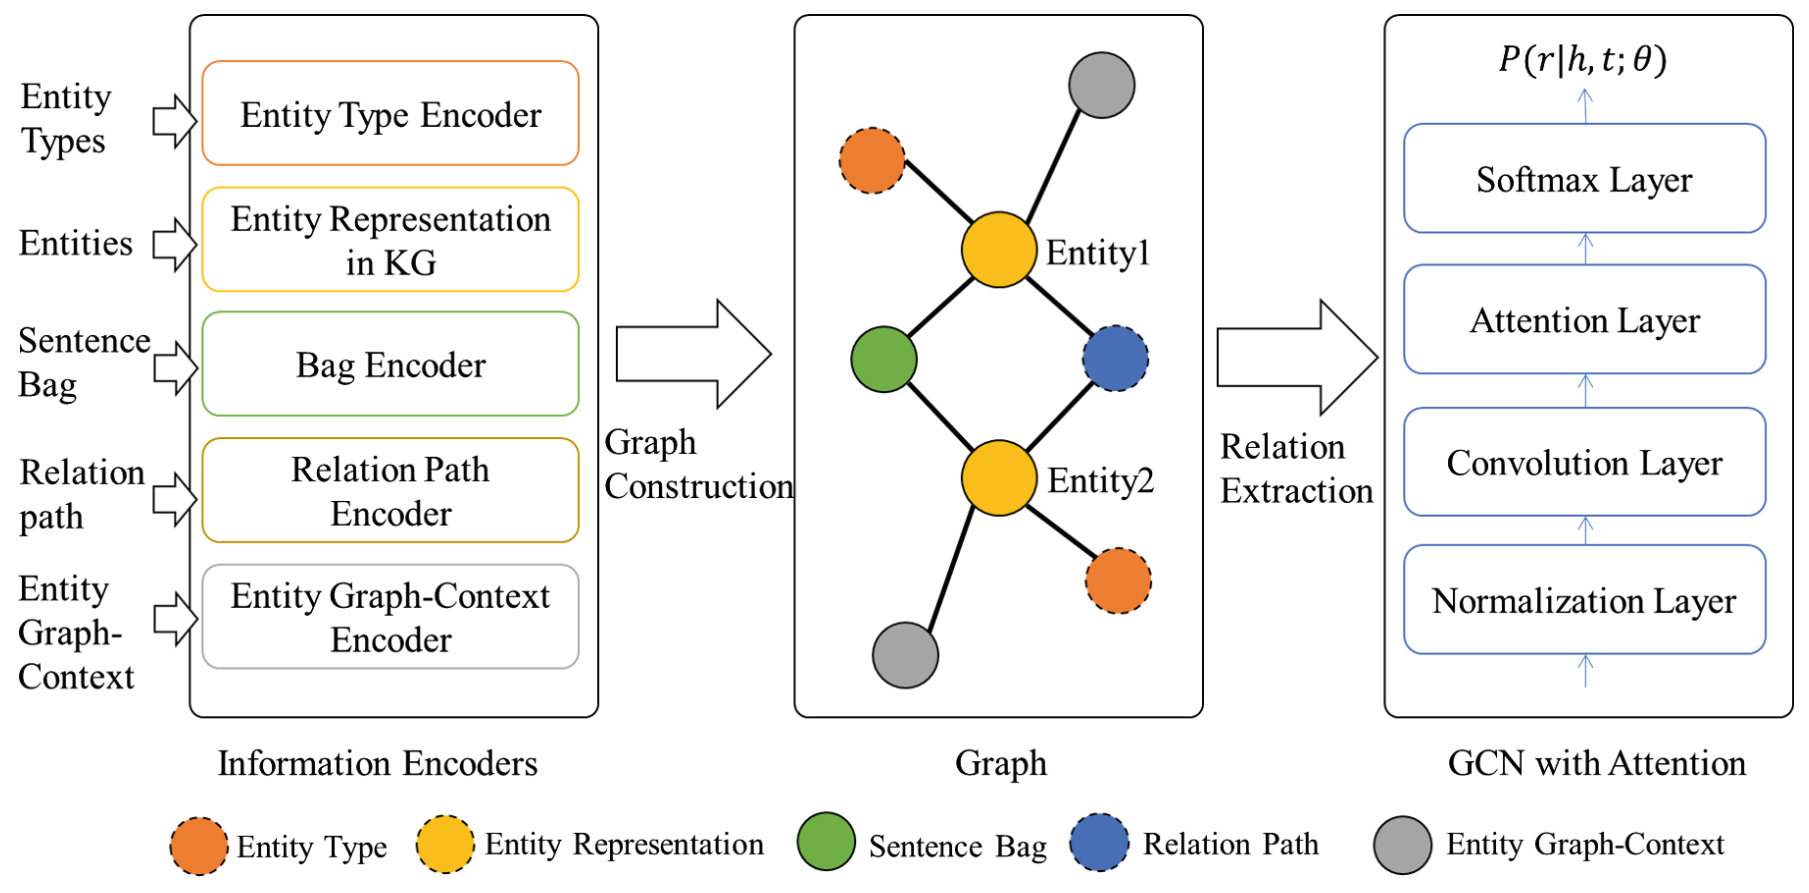
\includegraphics[scale=0.25]{figures/architecture.PNG}
	\caption{The Architecture}
	\label{fig:arch}
\end{figure}

\newpar
Before the process, from a given DS generated data set $D = \{S_{(x_i,y_i)}|,i = 1,2,...\}$, the background information from KG for every entity pair $(x_i, y_i)$ is extracted and stored in a different data set $\mathbb{I} = \{I_{(x_1,y_1)},I_{(x_2,y_2)},...\}$. Label of each instance corresponds to the label of $S_{(x_i, y_i)}$ during the extraction. 

\section{Information Encoding}
Following encoders\ref{fig:infenc} are used to learn the features and create vectors. These feature vectors are useful in creation of hybrid graph.

\begin{figure}[h!]
	\centering
	\includegraphics[scale=0.5]{figures/infoenc.PNG}
	\caption{Information Encoding}
	\label{fig:infenc}
\end{figure}

\subsubsection{Entity Encoder} 
Every entity $e_i$ is given a real-value vector $\txtb{e}_i$ representation with a dimension $d_e$. Pre-trained PTransE model was used for getting all entity embeddings, as it can capture a KG's path information efficiently. From the Fig.\ref{fig:infenc} from the given sentence all the entities are extracted such as John Doe, Jane doe and John Doe Inc. In this example, this encoder identifies Jane and Jane Doe as a single entity. A single vector of all entities will be the output.

\subsubsection{Sentence Bag Encoder}
Sentence Bag encoding is performed using a variant of LSTM, Bi-LSTM model to get the vector representation $\txtb{s}_i \in \mathbb{R}^{d_s}$ for any sentence $s_i \in S_{h,t}$ where $\left(h,t\right)$ is the entity pair. $d_s$ is the sentence embedding size. Finally $\txtb{S}_{\left(h,t\right)} \in \mathbb{R}^{d_s}$ is the sentence bag representation obtained by the process of summation of all vectors $\txtb{s}_i$ that have different individual weights. The authors Duan et al.\cite{duan2019hybrid} suggests to use a relevant model depending on the data, as long as it can represent the semantics of the given sentence. 

\subsubsection{Entity Type Encoder}
For each entity $e$, along with its entity type $y_e \in \txti{T}$ is identified using one-hot encoding. \txti{T} is the set of all entity types. A representation matrix, $\txtb{M}_y \in \mathbb{R}^{|\txti{T}| \times d_t}$ is used dynamically, to store the entity type distribution representation. $d_t$ is the entity type embedding size. Unlike entity and sentence bag encoders, entity type encoder encodes each entity type as a whole vector. For $n$ entities, there will be $\txtb{n}$ entity type vectors.

\subsubsection{Relation Path Encoder}
All the relation paths are concatenated and given as an input to the LSTM model. Entity embedding and sentence bag embedding for a sentence is concatenated and given as input to an LSTM cell\ref{ch:concepts}. 

\begin{figure}[h!]
	\centering
	\includegraphics[scale=0.2]{figures/LSTMarchit.PNG}
	\label{fig:lstmarchit}
\end{figure}

\begin{figure}[h!]
	\centering
	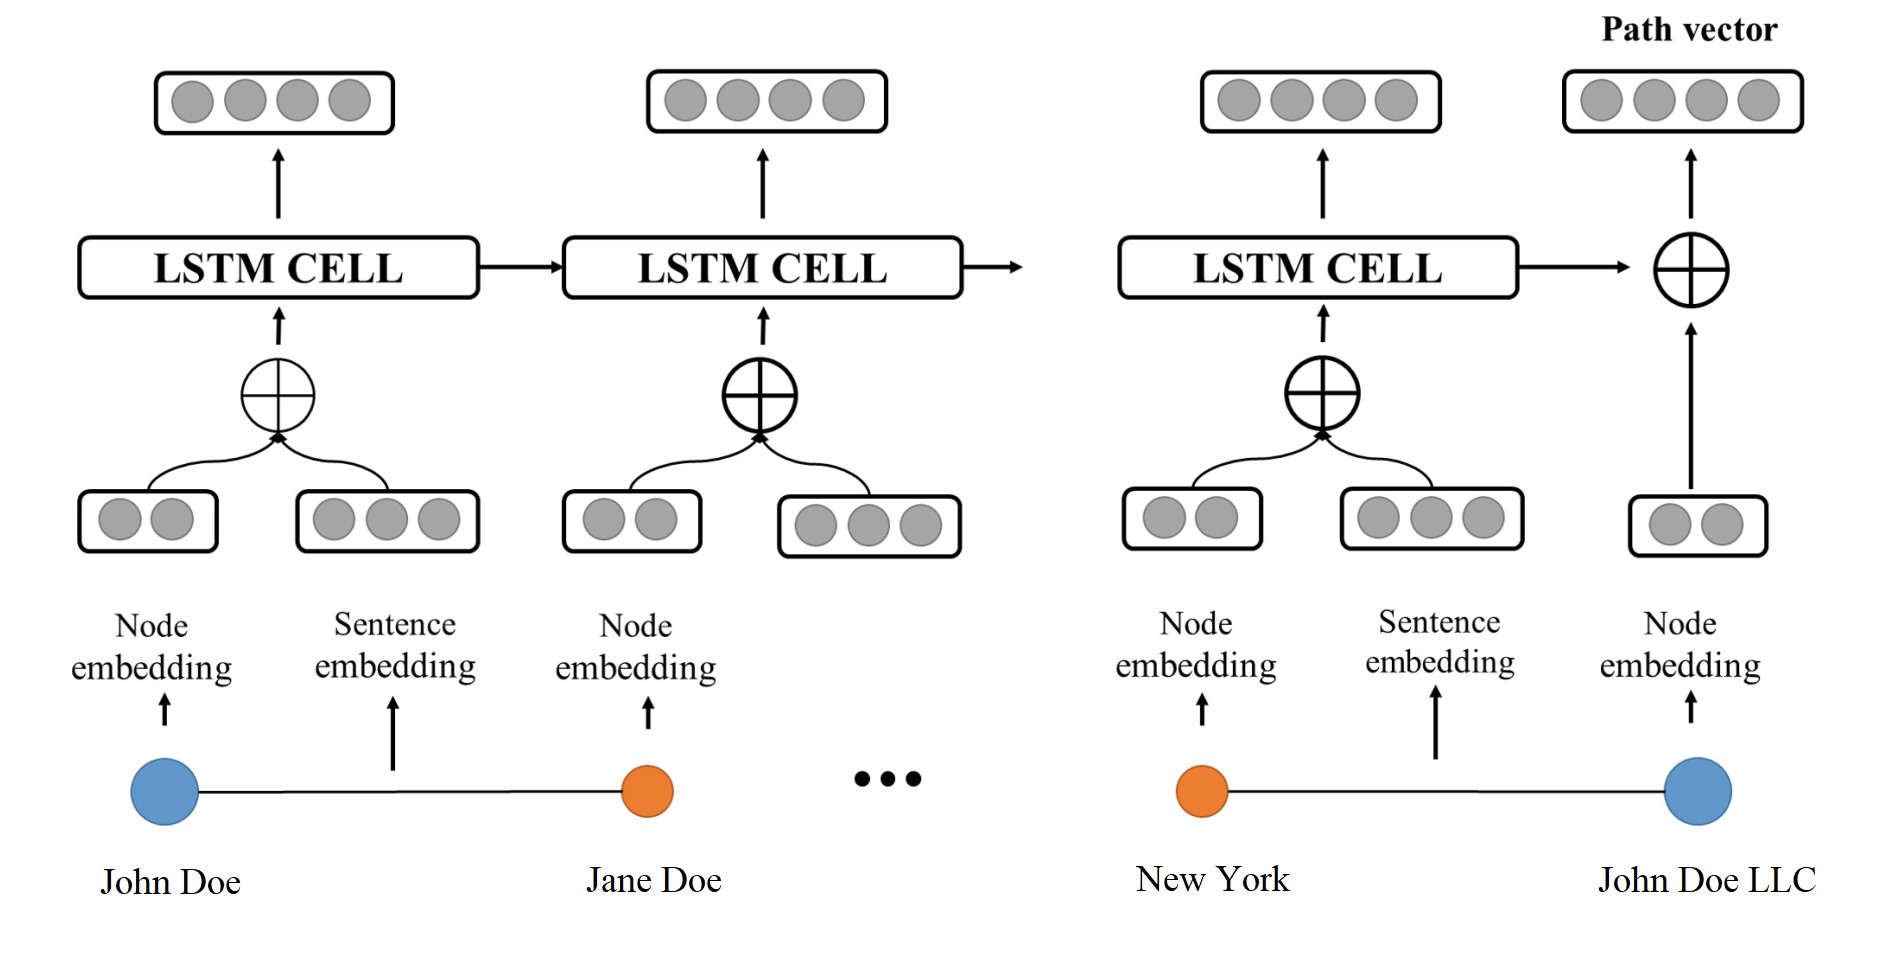
\includegraphics[scale=0.3]{figures/LSTM.PNG}
	\caption{Relation Path Encoder}
	\label{fig:lstm}
\end{figure}

\section{Hybrid Graph Construction}

\begin{figure}[h!]
	\centering
	\includegraphics[scale=0.5]{figures/grapgconc.PNG}
	\caption{Hybrid Graph}
	\label{fig:grapgconc}
\end{figure}

By utilizing the vector information from previous stage, each vector can be embedded into a Hybrid Graph(HG) where each node represents a vector. From the Fig.\ref{fig:grapgconc}, different types of feature vectors are represented with a separate color. Given a sentence, Entity vectors for $John Doe$ and $John Doe Inc$. are connected using the sentence bag embedding. if there is a relation path embedding corresponding to FounderOf relation, then the node gets connected to its adjacent nodes. Similarly for entity types, if there exists a vector, then they get connected. This example is an abstract representation of HG and there may be empty nodes for those entities that do not have sufficient information. In real-time, the HG is much more complex and sparse. There are no suitable Machine Learning or Deep Learning techniques to calculate or analyze this HG. To counter this, authors Duan et al.\cite{duan2019hybrid} uses a 3D matrix to represent the graph. First matrix is a degree matrix that represents the degree of each node. This matrix controls the information propagation on the graph. Second matrix is a adjacent matrix that stores node feature. Node feature is a encoder vector in adjacent matrix which describes which nodes are connected. 

\section{GCN with attention}

 
 
\begin{figure}[h!]
	\centering
	\includegraphics[scale=0.5]{figures/GCNatt.PNG}
	\caption{Layers of a GCN}
	\label{fig:GCNatt}
\end{figure}

